%%%% Paramétrage du TD %%%%
\def\xxnumchapitre{Chapitre 1 \vspace{.2cm}}
\def\xxchapitre{\hspace{.12cm} Découverte de l'algorithmique et de la programmation}

\def\xxcompetences{%
\textsl{%
\textbf{Savoirs et compétences :}\\
\vspace{-.4cm}
\begin{itemize}[label=\ding{112},font=\color{bleuxp}] 
\item .
%\item \textit{Mod3.C2 : } pôles dominants et réduction de l’ordre du modèle : principe, justification
%\item \textit{Res2.C4 : } stabilité des SLCI : définition entrée bornée -- sortie bornée (EB -- SB)	
%\item \textit{Res2.C5 : } stabilité des SLCI : équation caractéristique	
%\item \textit{Res2.C6 : } stabilité des SLCI : position des pôles dans le plan complexe
%\item \textit{Res2.C7 : } stabilité des SLCI : marges de stabilité (de gain et de phase)
\end{itemize}
}}


\def\xxfigures{
%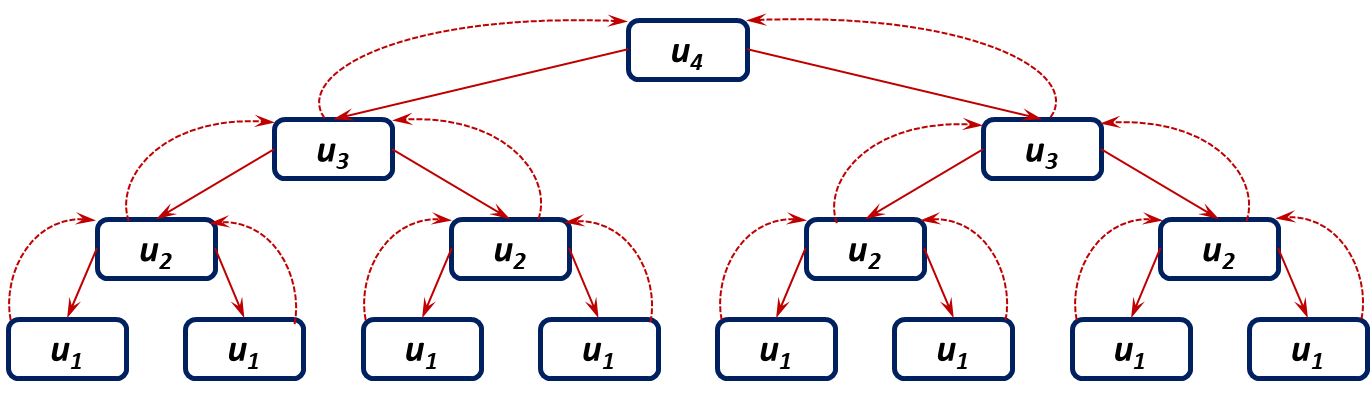
\includegraphics[width=3cm]{fig_01}\\
%\textit{}
}%figues de la page de garde

\def\xxtitreexo{Applications -- Bases}
\def\xxsourceexo{}
\def\xxactivite{{ Application 01} \ifprof  -- Corrigé \else \fi}

%\iflivret
\input{\repRel/Style/pagegarde_TD}
%\else
%\pagestyle{empty}


%%%%%%%% PAGE DE GARDE COURS
\ifcours
\begin{tikzpicture}[remember picture,overlay]
\node at (current page.north west)
{\begin{tikzpicture}[remember picture,overlay]
\node[anchor=north west,inner sep=0pt] at (0,0) {\includegraphics[width=\paperwidth]{\thechapterimage}};
\draw[anchor=west] (-2cm,-8cm) node [line width=2pt,rounded corners=15pt,draw=ocre,fill=white,fill opacity=0.6,inner sep=40pt]{\strut\makebox[22cm]{}};
\draw[anchor=west] (1cm,-8cm) node {\huge\sffamily\bfseries\color{black} %
\begin{minipage}{1cm}
\rotatebox{90}{\LARGE\sffamily\textsc{\color{ocre}\textbf{\xxnumpartie}}}
\end{minipage} \hfill
\begin{minipage}[c]{14cm}
\begin{titrepartie}
\begin{flushright}
\renewcommand{\baselinestretch}{1.1} 
\Large\sffamily\textsc{\textbf{\xxpartie}}
\renewcommand{\baselinestretch}{1} 
\end{flushright}
\end{titrepartie}
\end{minipage} \hfill
\begin{minipage}[c]{3.5cm}
{\large\sffamily\textsc{\textbf{\color{ocre} \discipline}}}
\end{minipage} 
 };
\end{tikzpicture}};
\end{tikzpicture}


\begin{tikzpicture}[overlay]
\node[shape=rectangle, 
      rounded corners = .25 cm,
	  draw= ocre,
	  line width=2pt, 
	  fill = ocre!10,
	  minimum width  = 2.5cm,
	  minimum height = 3cm,] at (18cm,0) {};
\node at (17.7cm,0) {\rotatebox{90}{\textbf{\Large\color{ocre}{\classe}}}};
%{};
\end{tikzpicture}

\vspace{3.5cm}

\begin{tikzpicture}[remember picture,overlay]
\draw[anchor=west] (-2cm,-6cm) node {\huge\sffamily\bfseries\color{black} %
\begin{minipage}{2cm}
\begin{center}
\LARGE\sffamily\textsc{\color{ocre}\textbf{\xxactivite}}
\end{center}
\end{minipage} \hfill
\begin{minipage}[c]{15cm}
\begin{titrechapitre}
\renewcommand{\baselinestretch}{1.1} 
\Large\sffamily\textsc{\textbf{\xxnumchapitre}}

\Large\sffamily\textsc{\textbf{\xxchapitre}}
\vspace{.5cm}

\renewcommand{\baselinestretch}{1} 
\normalsize\normalfont
\xxcompetences
\end{titrechapitre}
\end{minipage}  };
\end{tikzpicture}
\vfill

\begin{flushright}
\begin{minipage}[c]{.3\linewidth}
\begin{center}
\xxfigures
\end{center}
\end{minipage}\hfill
\begin{minipage}[c]{.6\linewidth}
\startcontents
\printcontents{}{1}{}
\end{minipage}
\end{flushright}

\begin{tikzpicture}[remember picture,overlay]
\draw[anchor=west] (4.5cm,-.7cm) node {
\begin{minipage}[c]{.2\linewidth}
\begin{flushright}

\includegraphics[width=2cm]{png/logoCC}
\end{flushright}
\end{minipage}
\begin{minipage}[c]{.2\linewidth}
\textsl{\xxauteur} \\
\textsl{\classe}
\end{minipage}
 };
\end{tikzpicture}
\newpage
\pagestyle{fancy}

\newpage
\pagestyle{fancy}

\else
\fi


%%%%%%%% PAGE DE GARDE TD
\iftd
%\begin{tikzpicture}[remember picture,overlay]
%\node at (current page.north west)
%{\begin{tikzpicture}[remember picture,overlay]
%\draw[anchor=west] (-2cm,-3.25cm) node [line width=2pt,rounded corners=15pt,draw=ocre,fill=white,fill opacity=0.6,inner sep=40pt]{\strut\makebox[22cm]{}};
%\draw[anchor=west] (1cm,-3.25cm) node {\huge\sffamily\bfseries\color{black} %
%\begin{minipage}{1cm}
%\rotatebox{90}{\LARGE\sffamily\textsc{\color{ocre}\textbf{\xxnumpartie}}}
%\end{minipage} \hfill
%\begin{minipage}[c]{13.5cm}
%\begin{titrepartie}
%\begin{flushright}
%\renewcommand{\baselinestretch}{1.1} 
%\Large\sffamily\textsc{\textbf{\xxpartie}}
%\renewcommand{\baselinestretch}{1} 
%\end{flushright}
%\end{titrepartie}
%\end{minipage} \hfill
%\begin{minipage}[c]{3.5cm}
%{\large\sffamily\textsc{\textbf{\color{ocre} \discipline}}}
%\end{minipage} 
% };
%\end{tikzpicture}};
%\end{tikzpicture}

%%%%%%%%%% PAGE DE GARDE TD %%%%%%%%%%%%%%%
%\begin{tikzpicture}[overlay]
%\node[shape=rectangle, 
%      rounded corners = .25 cm,
%	  draw= ocre,
%	  line width=2pt, 
%	  fill = ocre!10,
%	  minimum width  = 2.5cm,
%	  minimum height = 2.5cm,] at (18.5cm,0) {};
%\node at (17.7cm,0) {\rotatebox{90}{\textbf{\Large\color{ocre}{\classe}}}};
%%{};
%\end{tikzpicture}

% PARTIE ET CHAPITRE
%\begin{tikzpicture}[remember picture,overlay]
%\draw[anchor=west] (-1cm,-2.1cm) node {\large\sffamily\bfseries\color{black} %
%\begin{minipage}[c]{15cm}
%\begin{flushleft}
%\xxnumchapitre \\
%\xxchapitre
%\end{flushleft}
%\end{minipage}  };
%\end{tikzpicture}

% Bandeau titre exo
\begin{tikzpicture}[remember picture,overlay]
\draw[anchor=west] (-2cm,-4cm) node {\huge\sffamily\bfseries\color{black} %
\begin{minipage}{5cm}
\begin{center}
\LARGE\sffamily\color{ocre}\textbf{\textsc{\xxactivite}}

\begin{center}
\xxfigures
\end{center}

\end{center}
\end{minipage} \hfill
\begin{minipage}[c]{12cm}
\begin{titrechapitre}
\renewcommand{\baselinestretch}{1.1} 
\large\sffamily\textbf{\textsc{\xxtitreexo}}

\small\sffamily{\textbf{\textit{\color{black!70}\xxsourceexo}}}
\vspace{.5cm}

\renewcommand{\baselinestretch}{1} 
\normalsize\normalfont
\xxcompetences
\end{titrechapitre}
\end{minipage}  };
\end{tikzpicture}
\else
\fi


%%%%%%%% PAGE DE GARDE FICHE
\iffiche
\begin{tikzpicture}[remember picture,overlay]
\node at (current page.north west)
{\begin{tikzpicture}[remember picture,overlay]
\draw[anchor=west] (-2cm,-3.25cm) node [line width=2pt,rounded corners=15pt,draw=ocre,fill=white,fill opacity=0.6,inner sep=40pt]{\strut\makebox[22cm]{}};
\draw[anchor=west] (1cm,-3.25cm) node {\huge\sffamily\bfseries\color{black} %
\begin{minipage}{1cm}
\rotatebox{90}{\LARGE\sffamily\textsc{\color{ocre}\textbf{\xxnumpartie}}}
\end{minipage} \hfill
\begin{minipage}[c]{14cm}
\begin{titrepartie}
\begin{flushright}
\renewcommand{\baselinestretch}{1.1} 
\large\sffamily\textsc{\textbf{\xxpartie} \\} 

\vspace{.2cm}

\normalsize\sffamily\textsc{\textbf{\xxnumchapitre -- \xxchapitre}}
\renewcommand{\baselinestretch}{1} 
\end{flushright}
\end{titrepartie}
\end{minipage} \hfill
\begin{minipage}[c]{3.5cm}
{\large\sffamily\textsc{\textbf{\color{ocre} \discipline}}}
\end{minipage} 
 };
\end{tikzpicture}};
\end{tikzpicture}


\begin{tikzpicture}[overlay]
\node[shape=rectangle, 
      rounded corners = .25 cm,
	  draw= ocre,
	  line width=2pt, 
	  fill = ocre!10,
	  minimum width  = 2.5cm,
	  minimum height = 2.5cm,] at (18.5cm,0.5cm) {};
%	  minimum height = 2.5cm,] at (18.5cm,0cm) {};
\node at (17.7cm,0.5) {\rotatebox{90}{\textsf{\textbf{\large\color{ocre}{\classe}}}}};
%{};
\end{tikzpicture}

\else
\fi



%\fi

\setlength{\columnseprule}{.1pt}

\pagestyle{fancy}
\thispagestyle{plain}


\vspace{4.5cm}

\def\columnseprulecolor{\color{bleuxp}}
\setlength{\columnseprule}{0.4pt} 

%%%%%%%%%%%%%%%%%%%%%%%




\ifprof
\vspace{1cm}
\else
\begin{multicols}{2}
\fi

\subsection*{Initiation à l'implémentations de fonctions}
\setcounter{numques}{0}

\exer{Structures conditionnelles}

\question{Implémenter une fonction \texttt{est\_plus\_grand(a:int,b:int)-> bool} renvoyant \texttt{True} si $a>b$, \texttt{False} sinon. }



\question{\'Ecrire une fonction \texttt{neg(b)} qui renvoie la négation du booléen \texttt{b} sans utiliser \texttt{not}.}

\question{\'Ecrire une fonction \texttt{ou(a,b)} qui renvoie le ou logique des booléen \texttt{a} et \texttt{b} sans utiliser \texttt{not}, \texttt{or} ni \texttt{and}.}

\question{\'Ecrire une fonction \texttt{et(a,b)} qui renvoie le et logique des booléen \texttt{a} et \texttt{b} sans utiliser \texttt{not}, \texttt{or} ni \texttt{and}.}

%\subsubsection*{Implémentations de fonctions prenant des listes en argument}

\exer{Un tout petit peu d'arithmétique}

\question{Implémenter la fonction \textvtt{unite(n:int)->int} renvoyant le chiffre des unités de l'entier \texttt{n}.}


\begin{lstlisting}
>>> unite(123)
	3
\end{lstlisting}

\question{Implémenter la fonction \textvtt{dizaine(n:int)->int} renvoyant le chiffre des dizaines de l'entier \texttt{n}.}

\begin{lstlisting}
>>> dizaine(123)
	2
\end{lstlisting}

\question{Implémenter la fonction  \\ \textvtt{unites\_base8(n:int)->int} renvoyant le chiffre des unités de l'entier \texttt{n} en base 8.}

\exer{Liste de zéros}

\question{Implémenter la fonction \textvtt{zeros\_01(n:int)->list} permettant de générer une liste de \texttt{n 0}. On utilisera une boucle \texttt{while}.}

\begin{lstlisting}
>>> zeros_01(4)
	[0,0,0,0]
\end{lstlisting}

\question{Implémenter la fonction \textvtt{zeros\_02(n:int)->list} permettant de générer une liste de \texttt{n 0}. On utilisera une boucle \texttt{for}.}

\question{Implémenter la fonction \textvtt{zeros\_03(n:int)->list} permettant de générer une liste de \texttt{n 0}. On utilisera une boucle \texttt{while}. On génera cette liste << en compréhension >> (sans boucle \texttt{for} ou \texttt{while} explicite).}

\exer{Liste d'entiers}

\question{Implémenter la fonction \textvtt{entiers\_01(n:int)->list} permettant de générer la liste des entiers compris entre 0 inclus et \texttt{n} exclus. On utilisera une boucle \texttt{while}.}

\begin{lstlisting}
>>> entiers_01(4)
	[0,1,2,3]
\end{lstlisting}

\question{Implémenter la fonction \textvtt{entiers\_02(n:int)->list} permettant de générer la liste des entiers compris entre 0 inclus et \texttt{n} exclus. On utilisera une boucle \texttt{for}.}


\question{Implémenter la fonction \textvtt{entiers\_03(n:int)->list} permettant de générer la liste des entiers compris entre 0 inclus et \texttt{n} exclus. On génera cette liste << en compréhension >> (sans boucle \texttt{for} ou \texttt{while} explicite).}

\question{\'Ecrire une fonction \textvtt{carres(n:int)->list} qui prend en argument un entier naturel \texttt{n} et qui renvoie la liste des \texttt{n} premiers carrés d'entiers, en commençant par $0$.}

\question{\'Ecrire une fonction \textvtt{somme\_racine(n:int)->float} permettant de calculer la somme des racines carrées des n premiers entiers naturels non nuls.}

\exer{Notion d'effet de bords}

On cherche à écrire une fonction prenant en argument une liste d'entiers (non vide) et incrémentant de $1$ le premier élément de cette liste.

\question{\'Ecrire une telle fonction \textvtt{incr\_sans\_effet\_de\_bord(L:list)->list}, qui ne modifie pas la liste initiale et renvoie en sortie une nouvelle liste.}

\begin{lstlisting}
>>> L = [1,2,3]
>>> LL = incr_sans_effet_de_bord(L)
>>> print(L)
    [1,2,3]
>>> print(LL)
    [2,2,3]
\end{lstlisting}


\question{\'Ecrire une telle fonction \textvtt{incr\_avec\_effet\_de\_bord(L:list)-> None}, qui modifie la liste initiale et ne renvoie rien en sortie (ponctuer par un \texttt{return None}).}

\begin{lstlisting}
>>> L = [1,2,3]
>>> LL = incr_sans_effet_de_bord(L)
>>> print(L)
    [2,2,3]
>>> print(LL)
    None
\end{lstlisting}


\exer{Structures itératives}

\question{\'Ecrire la fonction \textvtt{somme\_inverse(n:int)->float} calculant la somme des inverses des \texttt{n} premiers entiers non nuls.}


\exer{Un petit peu de géométrie}

\question{Implémenter la fonction \textvtt{norme(A:list,B:list)->float} permettant calculer la norme du vecteur $\vect{AB}$ dans $\mathbb{R}^3$. Chacun des points sera constitué de la liste de ses coordonnées (par exemple \texttt{A=[xA,yA,zA]}).}

\question{Implémenter la fonction \textvtt{prod\_vect(u:list, v:list)->float} permettant calculer le produit vectoriel $\vect{u}\wedge \vect{v}$ dans $\mathbb{R}^3$.}



\exer{Suites d'entiers}

\question{Implémenter la fonction \textvtt{impairs(n:int)->list} permettant de générer la liste des \texttt{n} premiers entiers naturels impairs.}

\question{Implémenter la fonction \textvtt{multiples\_5(d:int, f:int)->list} permettant de générer la liste de tous les multuples de 5 compris entre \texttt{d} et \texttt{f} (bornes incluses si se sont des multiples de 5).}

\question{Implémenter la fonction \textvtt{cube(f:int)->list} permettant de générer la liste de tous les cubes d'entiers naturels inférieurs ou égaux à \texttt{f} (inclus si \texttt{f} est un cube).}


\exer{Un petit peu de statistiques}

\question{\'Ecrire une fonction \textvtt{moy\_extr(L:list)->float} qui prend en argument une liste \texttt{L} et renvoie en sortie la moyenne du premier et du dernier élément de \texttt{L}.}

\question{\'Ecrire une fonction \texttt{moyenne(L:list)->float} qui prend en argument une liste \texttt{L} et renvoie la moyenne des éléments de \texttt{L}.}

\question{\'Ecrire une fonction \textvtt{ecart\_type(L:list)->float} qui prend en argument une liste \texttt{L} et renvoie l'éacrt type des données : en notant $\overline{x}$ la moyenne des échantillons, on a  $\sigma = \sqrt{\dfrac{1}{n}\sum\limits_{i=1}^n \left(x_i^2  - \overline{x}\right)}$.}



\exer{Chaînes de caractères}

\question{\'Ecrire une fonction \texttt{lettre(i:int)->str} qui prend en argument un entier \texttt{i} et renvoie la \texttt{i}\ieme\ lettre de l'alphabet.}

\ifprof
\else
\end{multicols}
\fi

